\documentclass[journal=jacsat,manuscript=article,layout=twocolumn]{achemso}
% packages
%\usepackage {lmodern}
\usepackage [version=4]{mhchem}
\usepackage [T1]{fontenc}
\usepackage {amsmath}
%\usepackage {multicols}
\usepackage {amssymb}
\usepackage {amsfonts}
\usepackage {graphicx}
%\usepackage {fullpage}
%\usepackage {gensymb}
%\usepackage {caption}
%\usepackage {subcaption}
\usepackage {array}
\newcolumntype{L}{>{\centering\arraybackslash}m{3cm}}
%\usepackage {nopageno}
%\usepackage {cite}
%\usepackage {setspace}
\usepackage {pdfpages}
\usepackage {fancyvrb}

%\usepackage[dvipsnames]{xcolor}

\graphicspath {{images/}}

\author{Justin Chao}
\email{justin_chao@utexas.edu}
\affiliation[The University of Texas at Austin]
{Department of Chemistry, The University of Texas at Austin, Austin, TX}
\author{William Canales}
\affiliation[The University of Texas at Austin]
{Department of Chemistry, The University of Texas at Austin, Austin, TX}


\title[Potentiometric Determination of Fluoride in Solutions]
{Potentiometric Determination of Fluoride in Solutions}
\abbreviations{ISE, CDTA}
\keywords{Potentiometry}

\begin {document} 
\begin {abstract} 

Concentrations of Fluoride ions were potentiometrically determined in samples of
tap water, bottled water, and mouthwash, to be 2.5 $\pm$ 0.53 ppm,
7.66 $\times$ 10$^6$ $\pm$ 3.96 $\times$ 10$^6$, and 7.598 $\times$ 10$^{-20}$
$\pm$ 4.283 $\times$ 10$^{-21}$ respectively by a calibration curve method using
an ion selective electrode. Fluoride concentrations were unable to be determinded using a method
of standard additions due to faulty instrumentation. Findings from the
calibration curve method, while precise, were deemed inaccurate and
unreasonable when compared to literature values, also due to faulty
instrumentation.

\end{abstract}

\section {Introduction}
This experiment aims to determine the concentration of fluoride ions in
solutions using potentiometric techniques. Fluoride is often added in city
sources of water to help aid in lowering rates of tooth decay in the general
population. Fluoride ion concentrations of greater than 1 ppm however, can lead
to the pitting of teeth and bone cancer.

\subsection {Potentiometry}
Potentiometry is a quantitative method of passively measuring the electric
potential of an electrochemical cell containing an analyte solution using two
electrodes: a reference electrode and an indicator electrode. Schematically, this
is illustrated in Figure 1.

\begin{figure}
    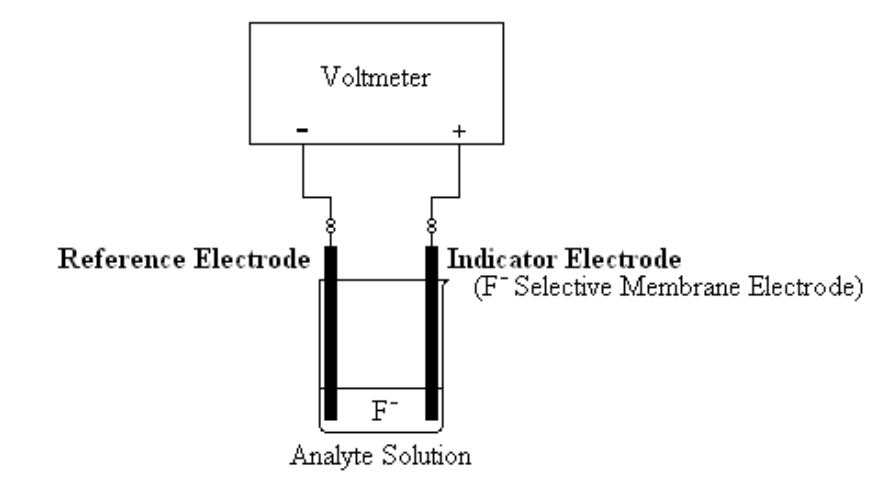
\includegraphics[scale=0.55]{meter}
    \caption {Potentiometric measurement system.}
    \label{fgr:example}
\end{figure}

The reference electrode has a potential which is
independent of the concentration of analyte ions in the solution and is
independent of temperature. The potential of the indicator electrode varies
depending on mainly the concentration, or activity, of analyte ions in solution
\cite{tartu}.

The difference in potential that occurs during measurement of the analyte
activity in solution between the reference and indicator electrodes provides an
assessment of the composition of the sample \cite{lab_man}.

The cell potential ($E_{cell}$) is measured using a voltmeter under
conditions of zero current flow. This limiting condition can be realized by
using a meter with an internal resistance of greater than 10$^{11}$ $\Omega$
\cite{nmt}.

Potentiometric measurements operate in a non-destructive manner to the sample being analyzed, and can be
conducted in an efficient and selective manner as well.

\subsection {Ion Selective Electrodes}
An ion selective electrode, or ISE, is a sensor that converts the activity of a specific ion in solution into
an electrical potential.
In this experiment, a Fluoride Ion Selective Membrane Double-Junction Electrode
is used, where the indicator and reference electrodes are built into a single
probe. Figure 2 diagrams the construction of such a probe \cite{nmt}.
\begin{figure}
    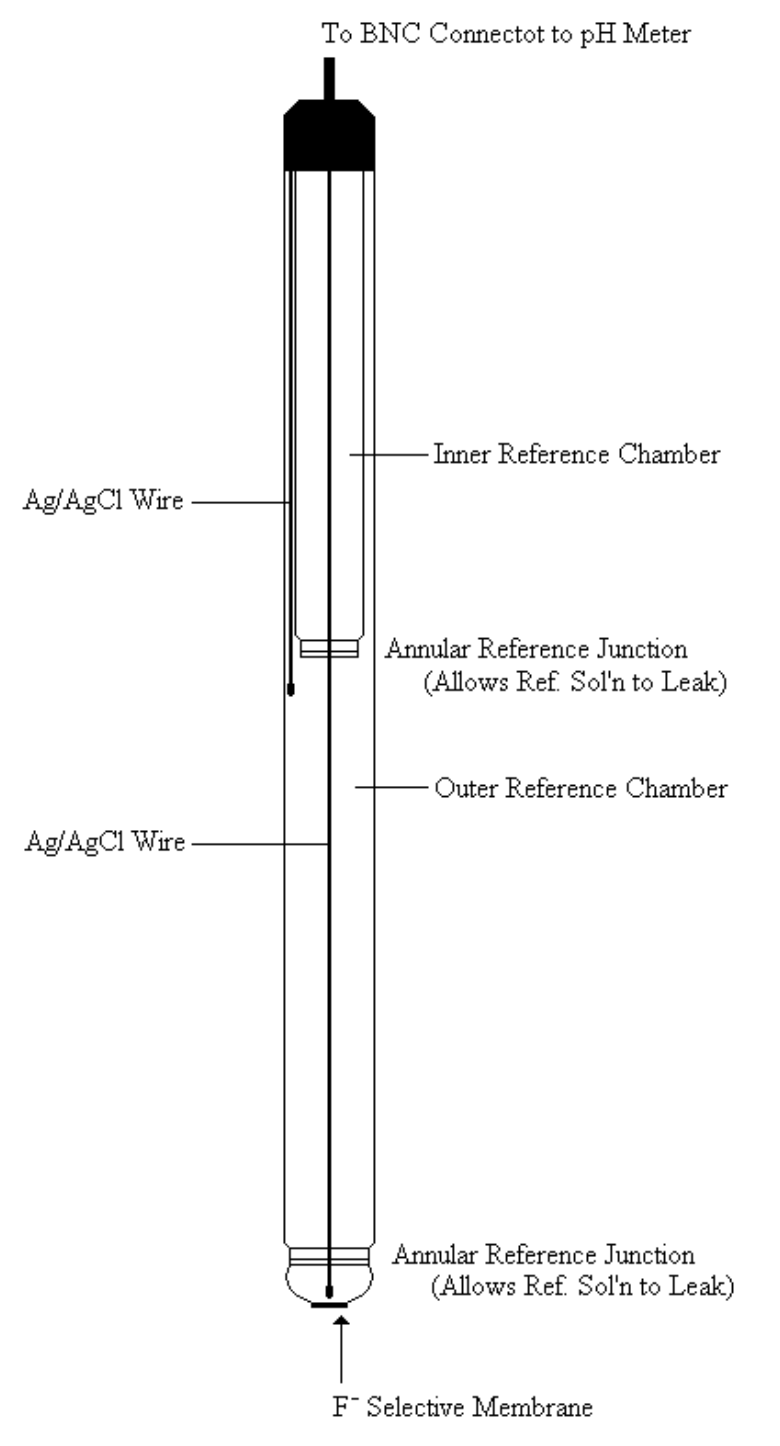
\includegraphics[scale=0.4]{probe}
    \caption{Diagram of a Fluoride Ion Selective Membrane
    Double-Junction Electrode.}
\end{figure}

The built-in reference electrode is a Ag|AgCl electrode which operates according
to the oxidation half-reaction given in Equation 1.
\begin{equation}
    \ce {Ag(s) + Cl-(aq) -> AgCl(s) + e-}
\end{equation}
Conversely, the indicator electrode is constructed from a AgCl|Ag electrode and a Fluoride
Ion Selective Membrane. 
The potential of the indicator electrode is controlled by the internal Cl$^-$
activity, which operates reductively as expressed in Equation 2.
\begin{equation}
    \ce {AgCl(s) + e- -> Ag(s) + Cl-(aq)}
\end{equation}

The membrane at the end of the indicator electrode selectively binds F$^-$ ions to both the exterior surface in
contact with the analyte solution, and the interior surface in contact with the
reference electrode. Figure 3 provides an illustration of this interaction.
\begin{figure}
    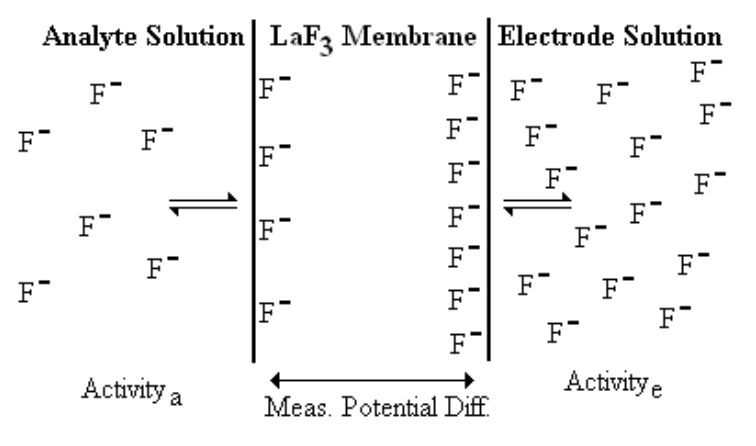
\includegraphics[scale=0.6]{membrane}
    \caption{Diagram of Fluoride Ion Selective Membrane in an analyte
    solution.}
\end{figure}

Due to the activity of the F$^-$ ion in the analyte solution being different from
that in the electrode solution, a potential difference is developed across the
membrane. 

The membrane used in the meter is composed of a lanthanum fluoride (LaF$_3$)
crystal doped with Europhium (II) ions to lower its electrical resistance and
facilitate ionic charge transport \cite{nmt}.
F$^-$ ions bind to the surface of the membrane according to Equation 3.
\begin{equation}
    \ce {LaF3(s) + F^-(aq) <=> LaF4^-(s)}
\end{equation}

The inside of the indicator electrode contains a solution of 0.1M NaCl and NaF.
The activity of these F$^-$ ions on the internal side of the membrane controls
the potential on the inner surface of the LaF$_3$ crystal.

The total potential of the cell can be written as a sum of the potentials of the
reference and the indicator electrodes, as noted in Equation 4.
\begin{equation}
    E_{cell} = E_{ind} - E_{ref} + E_{jnc}
\end{equation}
where $E_{jnc}$ is the potential that builds up at the junctions in the
of the cell's components (refer to Figure 2). Potential that builds up at these
junctions contribute to the largest source of error in most potentiometric
measurements \cite{nmt}.

\subsection {Calibration Curve Method}
A calibration curve is a method for determining the concentration of an analyte
in a sample by comparing the unknown to a series of standard samples of known
concentration. By plotting the signal received by the instruments vs. the concentration of a series of standard samples, a relationship can be found and
later used to interpolate the concentration of an unknown sample based on
instrument signal response. The concentrations of the standards used however
must lie within the working range of the instrument being used. In this
experiment, a calibration curve will be constructed by plotting the voltage read
from the multimeter vs. the log of the concentration of F$^-$ ions.

\subsection {Standard Addition Method}
The method of standard addition is another way of determining the concentration
of an analyte in a sample. This method is frequently used when the sample matrix
also contributes to the analytical signal, an effect known as the matrix effect
\cite{Harris}. Another factor that can affect the signal includes temperature.

In creating a standard addition curve, the signal intensity of the sample
solution is first measured, and then subsequent portions of a standard solution
are added in increasing volumes. The signal intensity is measured after each addition.
The optimal volume of each addition is that which gives the signal response a 1.5 to 3 times increase over
that of the initial sample \cite{aviv}.
A plot of the signal intensity vs. the added concentrations can then be constructed, and an extrapolation of
the line of best fit to the x-intercept will give the concentration of the analyte in question.
Figure 4 illustrates the preparation of four samples for determining the concentration of an unknown by standard
addition\cite{zellmer}.
\begin{figure}
    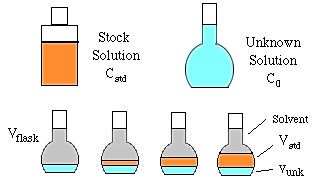
\includegraphics[scale=0.65]{stdadd}
    \caption{Preparation of four samples for the construction of a standard addition curve.}
\end{figure}
Since the method of standard addition is dependent upon data given from a
calibration curve, there is a propagation of error when using the standard addition
method.

\subsection {Total Ionic Strength Adjustment Buffer}
The Ion Selective Electrode used in this experiment is sensitive to hydroxide
ions when its concentration becomes greater than 10\% of the fluoride ions
present in solution, and therefore must be controlled with a buffer\cite{nmt}.
Total Ionic Strength Adjustment Buffer, or TISAB, is used to control the levels of OH$^-$
ions in solution, and consists of a mixture of NaOH, NaCl, glacial acetic acid,
and CDTA.

TISAB also keeps the pH of the solution buffered at 5.25\cite{nmt}. This keeps
F$^-$ ions from being protonated to form HF, as illustrated in Equation 5,
\begin{equation}
    \ce {F^-(aq) + H^+(aq) <=> HF(aq)} \\
\end{equation}
where pK$_a$ = 3.17.

Additionally, TISAB controls the ionic strength of the analyte solution and
keeps the total ionic strength at a high and constant value.
This is important since potentiometric measurements measure the activity of the
analyte, rather then the concentration. Since the activity coefficient
($\gamma_{F^-})$ is usually indeterminable, the ISE must be calibrated instead
against solutions of known concentration, rather than known activity. This
method only works if the ionic strength of the calibration standards and the
analyte solution are the same \cite{nmt}.

Finally, TISAB contains the complexing agent CDTA \\
(trans-1,2-cyclohexanedinitrilotetraacetic acid). This agent complexes with
Al$^{3+}$, Fe$^{3+}$, and other metal ions and prevents these metal ions from complexing with
F$^-$ ions and interfering with the potentiometric measurements. Equation 6
illustrates how Al$^{3+}$ can complex with F$^-$.
\begin{equation}
    \ce {Al^{3+}(aq) + 4F-(aq) <=> AlF4-(aq)}
\end{equation}

Figure 5 illustrates the structure of CDTA.
\begin{figure}
    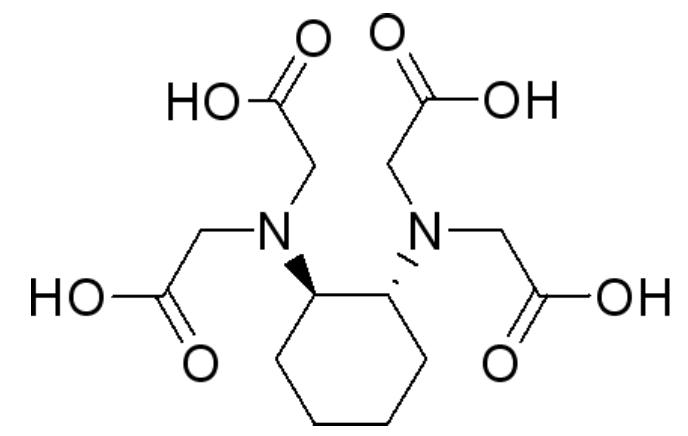
\includegraphics[scale=0.5]{cdta}
    \caption{Structure of CDTA.}
\end{figure}

\subsection {The Nernst Equation}
The dependence of potential between the electrodes can be expressed by the Nernst
equation, given in Equation 7 \cite{lab_man}.
\begin{equation}
    \begin {aligned}
    E_{ind} = E_{ref} - E_{jnc} + \frac{RT}{ZF}ln(a_i)
    \end {aligned}
\end{equation}
where \\
$E_{ind}$ = measured electrode potential \\
$E_{ref}$ = reference potential of the electrode \\
$E_{jnc}$ = junction potential \\
$R$ = universal gas constant (8.314 $\frac{J}{K*mol}$) \\
$F$ = Faraday constant (96,485 C/mol) \\
$T$ = temperature (K) \\
$Z$ = charge of the ion or number of electrons participating in the reaction \\
$a$ = ionic activity, where activity is a function of concentration (see
Equation 9).

For solutions with concentrations lower than 0.1 mol/L, activity can be 
approximated to concentration. Therefore, there exists a logarithmic
dependence between potential and activity of ions in solution.

Ionic strength, expressed in Equation 8, is a measure of the total ion concentration in solution. Ions
with more charge are counted more due to stronger electrostatic interactions
with other ions.
\begin{equation}
    I = \frac{1}{2}\sum_i = c_iz_i^2
\end{equation}
where \\
$I$ = ionic strength \\
$c$ = ion concentration \\
$z$ = ion charge

Equation 9 expresses the ionic activity as a function of ion concentration.
\begin{equation}
    a_i = \gamma_ic_i
\end{equation}
where \\
$a$ = ionic activity \\
$\gamma$ = activity coefficient

Using these relationships, Equation 7 can be rewritten as Equation 10.
\begin{equation}
    \begin{aligned}
        E_{ind} = &E_{ref} - E_{jnc} + \frac{RT}{ZF}ln(\gamma_{F^-})  \\
        &+ 2.303 \frac{RT}{ZF} log(c_{F-}) 
    \end{aligned}
\end{equation}
where \\
$\gamma_{F^-}$ = activity coefficient of the fluoride ion \\
$c_{F^-}$ = concentration of fluoride ions \\ 

Equation 10 can be generalized and rewritten as Equation 11 below.
\begin{equation}
    E_{ind} = K - 0.0592\times log(c_{F^-})
\end{equation}
where $K$ is a constant that is specific to the cell.

If interfering ions, such as OH$^-$, bind to the membrane surface of the
indicator electrode, these interactions must also be included in the activity
present, as illustrated in Equation 12.
\begin{equation}
    \begin{aligned}
        E_{ind} &= L - 0.0592  \\
        &\times log (c_{F^-} + k_{(F^-,OH^-)}c_{PH^-})
    \end{aligned}
\end{equation}
where $k_{(F^-,OH^-)}$ is the selectivity coefficient of the electrode towards
interference by OH$^-$ ions \cite{nmt}.

Inserting Equation 11 into Equation 7 and rearranging by conversion of $c_{F^-}$ to $pF$ gives Equation 13 below.
\begin{equation}
    \begin{aligned}
    pF &= -log (c_{F^-}) \\
    &= \frac{(E_{cell} - E_{jnc} - E_{ref} - L)}{0.0592} \\
    &= \frac{E_{cell} - K}{0.0592} 
    \end{aligned}
\end{equation}
where $K$ is a constant that is specific to the cell and can be determined by a
calibration. 
Equation 13 can then be rearranged to be expressed as Equation 14.
\begin{equation}
    E = (59.16) pF + K
\end{equation}

According to Equation 14, the measured potential should change by approximately
59 mV as the concentration of F$^-$ ions is changed by a factor of 10.

In determining the Fluoride content of an unknown solution by method of variable
volume standard addition, Equation 11 can be rearranged to give Equation 15
below.
\begin{equation}
\begin{aligned}
    E &= K + m\times log(c_{F^-}) \\
    c_{F^-} &= 10^{\frac{E-K}{m}}  \\
    &= \frac{10^{\frac{E}{m}}}{10^{\frac{K}{m}}}
\end{aligned}
\end{equation}
where $m$ is the slope of the calibration curve and $K$ is a constant.

The concentration of $F^-$ ions after any addition of the standard solution can
then be expressed by Equation 16.
\begin{equation}
    c_{F^-} = \frac{C_oV_o + C_{std}V_{std}}{V_o + V_{std}}
\end{equation}
where \\
$C_o$ is the initial concentration of fluoride ions before any standard is
added. \\
$V_o$ is the initial volume of the solution before any standard is added. \\
$C_{std}$ is the concentration of the standard solution. \\
$V_{std}$ is the volume of the standard solution that is added. 

Combining Equations 15 and 16 and rearranging gives Equation 17 in familiar
form of $y=b+mx$.
\begin{equation}
\begin{aligned}
    10^{\frac{E}{m}} (V_o + V_{std}) &= 10^{\frac{K}{m}}C_oV_o +
    10^{\frac{K}{m}}C_{std}V_{std} \\
    10^{\frac{E}{m}} V_{tot} &= 10^{\frac{K}{m}} C_oV_o +
    10^{\frac{K}{m}}C_{std}{V_{std}}
\end{aligned}
\end{equation}
where \\
$m$ = slope of the calibration curve (approximately -59 mV).  \\
$K$ = y-intercept of the calibration curve.


\section {Results}
The tap water sample used in this experiment came from a sink in the laboratory
room WEL 4.124 located at The University of Texas at Austin in Austin, TX.
The bottled water sample used was Ice Canyon. The mouthwash sample used was
Listerine. The multimeter probe used was \#10.

All plots were constructed using Gnuplot. Table 1 shows the potentials measured
for different levels of F$^-$ ion concentration. 

\begin{table}
    \caption{Calibration Curve Method Results}
    \begin{tabular}{L|L}
        \hline
        F$^-$ Ion Concentration (ppm) & Measured Potential (mV) \\
        \hline
        200 & 100.4 \\
        20 & 82.5 \\
        2 & 67.3 \\
        0.2 & 51.4 \\
        \hline
    \end{tabular}
\end{table}

Chart 1 shows the calibration curve generated by plotting the measured
potential vs. the log of the F$^-$ ion concentration. The equation of the line of
best fit, along with the correlation coefficient are shown. The line of best fit
was found using Gnuplot's "fit" command, which implements a nonlinear
least-squares method using the Marquardt-Levenberg algorithm. Please refer to
the Appendix for further details regarding the fit data.

\begin{chart}
    
\includegraphics[scale=0.35]{calibration} 
    \caption{Calibration Method Curve}
\end{chart}

Table 2 shows the measured potential readings for each unknown solution.
\begin{table}
    \caption{Measured Potential (mV) for Unknown Solutions}
    \begin{tabular}{c|c|c|c}
        \hline
        Unknown & Trial 1 & Trial 2 & Trial 3 \\
        \hline
        Tap Water & 64.2 & 65.5 & 65.8 \\
        Bottled Water & 108.3 & 112.5 & 110.5 \\
        Mouthwash & -72.5 & -72.3 & -72.1 \\
        \hline
    \end{tabular}
\end{table}

Using the equation generated from the calibration curve, the F$^-$ ion
concentrations in the tap water, bottled water, and mouthwash samples were
calculated. These values are listed in Table 3. Please refer to the Appendix for
detailed calculations of results and statistics.

\begin{table*}[t]
    \caption{Fluoride Ion Concentration in Unknown Samples as Determined by
    Calibration Curve Method.}
    \begin{tabular}{L|L|L|L}
        \hline
        & [F$^-$] (ppm) & [F$^-$] $\pm$ 95\% confidence interval & [F$^-$] $\pm$ 98\% confidence interval \\
        \hline
        \textbf{Tap Water}& 2.5 $\pm$ 0.53 & 2.5 $\pm$ 1.3 & 2.5 $\pm$ 2.1 \\
        \hline
        \textbf{Bottled Water} & 7.66 $\times$ 10$^6$ \hspace{2cm} $\pm$ 3.96 $\times$ 10$^6$ & 
        7.66 $\times$ 10$^6$ \hspace{2cm} $\pm$ 9.84 $\times$ 10$^6$ & 
        7.66 $\times$ 10$^6$ \hspace{2cm} $\pm$ 1.59 $\times$ 10$^7$ \\
        \hline
        \textbf{Mouthwash} & 7.598 $\times$ 10$^{-20}$ \hspace{2cm} $\pm$ 4.283 $\times$ 10$^{-21}$ & 
        7.598 $\times$ 10$^{-20}$ \hspace{2cm} $\pm$ 1.064 $\times$ 10$^{-20}$ & 
        7.598 $\times$ 10$^{-20}$ \hspace{2cm} $\pm$ 1.722 $\times$ 10$^{-20}$ \\
        \hline
    \end{tabular}
\end{table*}

Table 4 lists the measured potential readings for each sample using the standard
additions method.
\begin{table*}[t]
    \caption{Measured Potential (mV) for Samples using Standard
    Addition.}
    \begin{tabular}{L|L|L|L|L}
        \hline
        Flask & V$_{unknown}$ (mL) & V$_{standard}$ (mL) & V$_{total}$ (mL) & Measured Potential (mV) \\
        \hline
        \textbf{Tap Water} & & & & \\
        A & 1.0 & 0.5 & 10.0 & 36.9 \\
        B & 1.0 & 1.0 & 10.0 & 20.7 \\
        C & 1.0 & 2.0 & 10.0 & 2.1 \\
        D & 1.0 & 3.0 & 10.0 & -7.0 \\
        \hline
        \textbf{Mouthwash} & & & & \\
        A & 1.0 & 0.5 & 10.0 & -18.8 \\
        B & 1.0 & 1.0 & 10.0 & -22.9 \\
        C & 1.0 & 2.0 & 10.0 & -28.1 \\
        D & 1.0 & 3.0 & 10.0 & -31.2 \\
        \hline
    \end{tabular}
\end{table*}

Chart 2 shows the standard additions curve generated for the tap water sample.
\begin{chart}
    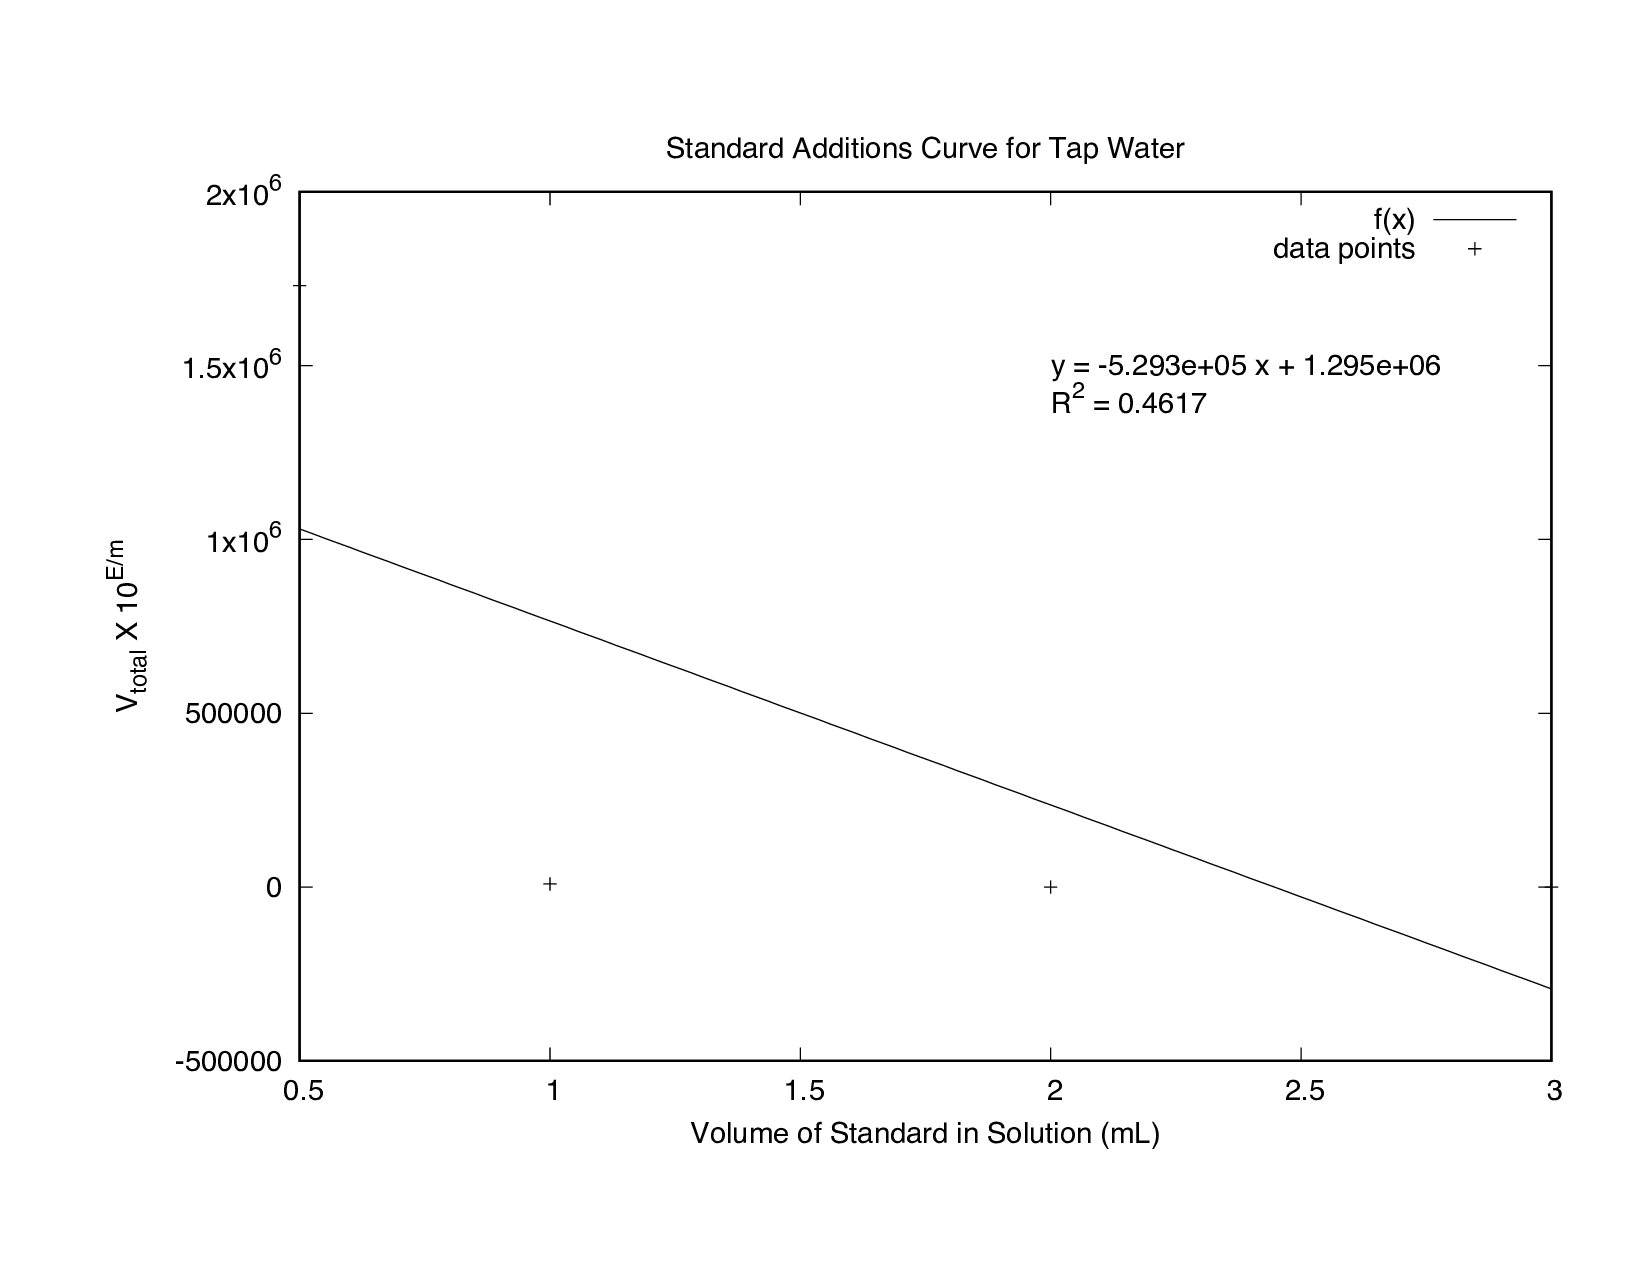
\includegraphics[scale=0.16]{std_tap}
    \caption{Standard Additions Curve for Tap Water Sample}
\end{chart}

Chart 3 shows the standard additions curve generated for the mouthwash sample.
\begin{chart}
    
\includegraphics[scale=0.36]{std_mouthwash} 
    \caption{Standard Additions Curve for Mouthwash Sample}
\end{chart}

A Grubbs' test for outliers was conducted for all datasets recorded, and no
outliers were detected with a significance level of $\alpha$ = 0.05.

The initial concentration of fluoride ions in the tap water and mouthwash
samples is deemed indeterminable from the data gathered using the method of
standard additions.

\section {Discussion}
Fluoride ion concentrations of greater than 1 ppm can lead to the pitting of
teeth and bone cancer.
The concentration of fluoride ions determined in the lab exceed safe levels of
fluoride concentration. It is immediately apparent that the values recorded in
this experiment are not reasonable and large sources of error are present.

[1] The most likely source of error may be due to a faulty multimeter or ISE probe. It is possible
that the multimeter used may not have been calibrated correctly either. While
the linear range of the fluoride ISE is reported to be 0.2 to 19,000 ppm
\cite{lab_man}, values obtained in this experiment deviate far outside these
limits.

Other sources of error include a contaminated TISAB buffer solution. Such a
contamination could cause inaccurate readings of F$^-$ ion activity to be
less than what they actually are due to inefficient complexing
by CDTA or a variable total ionic strength. 
A faulty TISAB solution could also cause pH values to deviate from
ideal values, giving rise to more F$^-$ ions becoming protonated in solution.

Contaminated glassware with residual anions or metal ions could also be a factor
in why F$^-$ ion concentrations were so low in the mouthwash sample, as residual
metal ions can complex with F$^-$ ions and anions can react with species in
solution, causing an imbalance in the equilibrium of F$^-$ ions. This imbalance
may result in an increased signal response and greater than actual concentration
values of F$^-$ ions in solution.

Human error is always a factor, and may be compounded due to multiple persons
preparing solutions and measuring signal intensities of samples.

The amount of fluoride in the mouthwash is reported to be 0.01\% (w/v), or 100
ppm \cite{lab_man}. The value obtained in this experiment was 7.598 $\times$ 10$^{-20}$. This
large discrepancy may be a result of the sources of error mentioned above.

[2] The value of $F^-$ concentration obtained for bottled water was 7.66 $\times$
10$^6$. This is not a reasonable value and is highly probably to be inaccurate.

[3] If an organic solvent was a contaminant in the solution, then a standard
addition method would be better suited for use in terms of data analysis, due to
the complexity of the matrix being analyzed. Signal response while constructing
a calibration curve could be affected by the organic species in solution.

[4] If TISAB was not added to the solutions prior to measurement, the measured
voltage on the multimeter would be lower than actual value, as metal cations
present in solution would complex with F$^-$ ions and prevent the ions from
exchanging across the ISE membrane. As a result, a lower concentration of F$^-$
ions would be reported by the multimeter.

[5] The solution must be constantly and consistently swirled to sure equal and
complete mixing of the TISAB buffer solution with the analyte solution to
prevent sources of error as mentioned previously. A well dispersed solution of
F$^-$ ions will also give the most accurate ion activity and exchange signal for
the analyte solution.

[6] Other methods for determining fluoride content in water include colorimetry. A
colorimetric method is based on the reaction of fluoride with a dark red
zirconium dye lake, which forms a colorless complex anion. This method results
in a bleaching of the red color by an amount that is proportional to the
fluoride ion concentration. As the amount of F$^-$ increases, the resulting
color becomes lighter. The color can then be photometrically analyzed using a
filter photometer or spectrophotometer \cite{colo}.
Colorimetric methods are susceptible to interfering species such as high
concentrations of alkalinity, aluminum, chloride, iron, phosphate, and sulfate.
Colorimetric methods are however, popular among dentists due to its low cost and
ease of implementation in the office \cite{burton}.

As illustrated in Figures 7 and 8, the standard addition curves generated in
this lab consist of a negative slope. This is a relationship that is contrary to
what is expected to happen, as a positive slope is the expected relationship
between the analytical signal vs. the concentration of added analyte.
Chart 4 illustrates such an expected standard addition calibration curve
relationship \cite{csun}.

\begin{chart}
    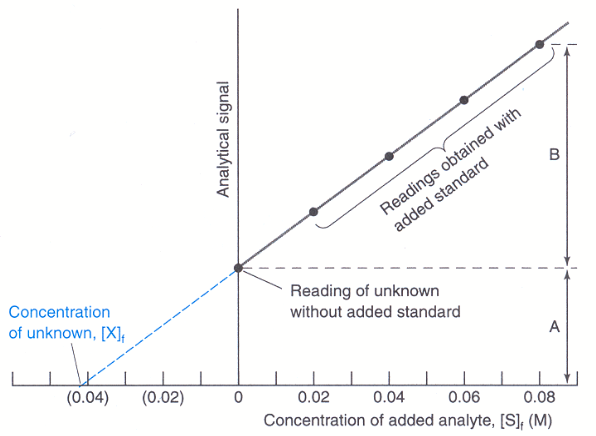
\includegraphics[scale=0.4]{std}
    \caption{General plot of a standard addition calibration curve.}
\end{chart}

Using such a standard addition curve, the F$^-$ ion concentration of an unknown
sample can be determined by extrapolating the line to the x-intercept. Using
equations derived from the Nernst equation, the x-intercept should be a negative
value. This is not the case with the standard addition curves generated in this
experiment. Therefore, the fluoride ion concentrations of the tap water and
mouthwash samples are deemed indeterminable by the standard addition curves
generated. The most likely source of error is a faulty multimeter, as described
previously.

According to the City of Austin Water Quality Report for the 2nd Quarter (Apr -
Jun), the Fluoride concentration tested at the Davis Water Treatment Plant was
0.20 ppm \cite{atx}. Compared with the value calculated in this experiment for tap water, 2.5 $\pm$ 0.53,
the results obtained in this experiment are not reasonable with what one might
expect to find in drinking water.

\section {Experimental}

Chemicals used include sodium fluoride (NaF) in concentrations of up to 2000 ppm and TISAB,
which consists of a mixture of NaOH, NaCl, glacial acetic acid, and CDTA. Sodium
% acetic acid formula, purity of TISAB %
fluoride is an irritant and is toxic in high concentrations. TISAB is an
irritant and is investigated to be mutagenic. Gloves should be worn and changed
often.
The instrument used is a fluoride ion selective membrane double-junction electrode composed of a
lanthanum fluoride (LaF$_3$) crystal doped with Europhium (II) ions, and
connected to a voltage reading multimeter.

Equal volumes of 4.0 mL of a 200 ppm, 20 ppm, 2 ppm, and 0.2 ppm fluoride
solution and 4.0 mL of a TISAB solution were volumetrically prepared and
measured with the fluoride ISE to generate a calibration curve.

Volumes of 4.0 mL each of the tap water, bottled water, and mouthwash samples
were prepared along with 4.0 mL of TISAB in each. The concentrations of fluoride
ions in each sample was determined using the previously generated calibration
curve.

Four samples consisting of 0.5 mL, 1.0 mL, 2.0 mL, and 3.0 mL of a standard 20
ppm F$^-$ solution were prepared. To each sample, 5.0 mL of TISAB and 1.0 mL of
the tap water sample was added. Finally, each sample was diluted to a total
volume of 10.0 mL. Another four samples were prepared in the same way with the
mouthwash sample. Using the fluoride ISE, the potential reading for each sample
was recorded and a standarad additions curve was constructed using relationships
derived from the Nernst equation (see Equation 17).

\section {Conclusion}
The results of this experiment are deemed unreasonable and the procedure should
be conducted again using a different multimeter and Fluoride ISE. Values for the
concentration of fluoride ion found in tap water, bottled water, and mouthwash
are inaccurate when compared to values found in literature. As the values
obtained in multiple trials are relatively precise, major sources of error may
include a faulty multimeter that may not have been calibrated correctly.

Other studies involving the use of ion selective electrodes includes one
conducted using a copper ISE to potentiometrically determine penicillamine in
pharmaceuticals. \cite{pen} This proposed method can determine Pen in an acetic
buffer of pH = 4 without pretreatment of the pharmaceuticals.  The determination
is based on the reaction between Pen and Cu$^{2+}$.


\begin {suppinfo}
\begin{itemize}
    \item File: cali\_data.csv, data file used to construct calibration curve.
    \item File: add\_data.csv, data file used to construct standard additions curves.
    \item Gnuplot fit and stats parameters for constructing calibration curve.
    \item Gnuplot fit and stats parameters for constructing standard additions
        curve for tap water sample.
    \item Gnuplot fit and stats parameters for constructing standard additions
        curve for mouthwash sample.
    \item City of Austin 2016 - 2nd Quarter Averages, Water Quality Report
        Summary
    \item Lab notebook pages with raw data and calculations.
\end{itemize}
\end {suppinfo}


\bibliography{fluoride.bib}


\onecolumn
\newpage
\VerbatimInput{cali_data.csv}
\vspace{5cm}
\VerbatimInput{add_data.csv}
\newpage
\VerbatimInput{cali.txt}
\newpage
\VerbatimInput{cali_stats.txt}
\newpage
\VerbatimInput{add_tap.txt}
\newpage
\VerbatimInput{add_tap_stats.txt}
\newpage
\VerbatimInput{add_mouthwash.txt}
\newpage
\VerbatimInput{add_mouthwash_stats.txt}
\newpage
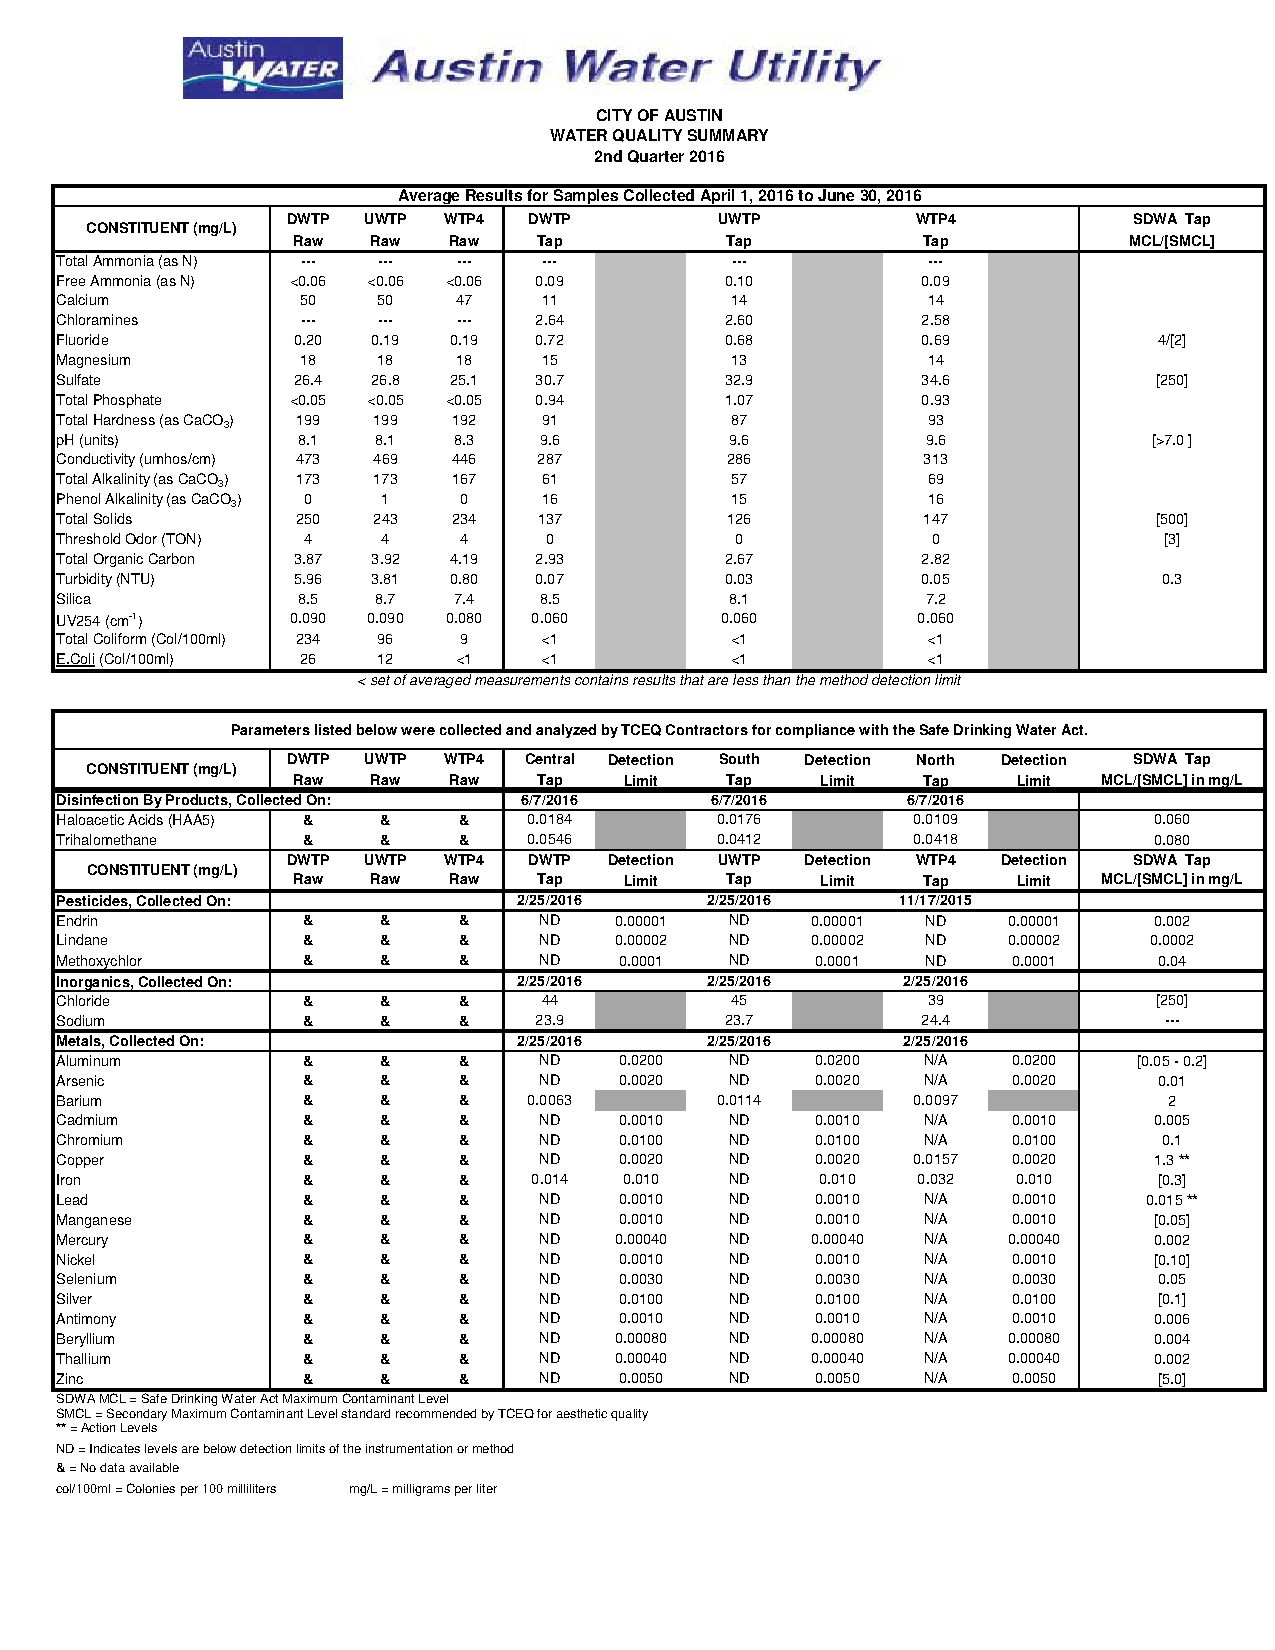
\includepdf[pages=-]{WQS.pdf}

\end {document}
